\section{Methods}\label{sec:methods}

\paragraph{Overview.}
\tool accepts long reads from a normal sample and one or more tumor samples from the same patient (Fig.~\ref{fig:overview}). After homopolymer compression~\cite{Li_2018}, \tool partitions reads into variable-length \textit{cores} across multiple granularity levels via locally consistent parsing (LCP)~\cite{lcpan,sv94a}. Core and core-pair frequencies capture sample coverage and tumor purity, defining minimum read-support thresholds. \tool then constructs a colored de~Bruijn-like graph~\cite{cortex} from these cores, tracking sample-specific read counts on each node (Fig.~\ref{fig:overview}a). After standard tip clipping and bubble popping~\cite{velvet}, \tool identifies edge pairs traversed exclusively by tumor reads as candidate somatic SV sites, detecting shared sites across multiple tumors only once (Fig.~\ref{fig:overview}b,c).

To place candidate sites on the reference genome, \tool extracts read subsequences (\textit{snippets}) bounded by normal-shared anchor cores from up to four supporting tumor reads. It maps snippets with minimap2~\cite{Li_2018} to short reference windows seeded by shared cores, and the alignments resolve breakpoints and SV types. In a second pass, \tool measures anchor-to-anchor distances across reads to detect cryptic normal support for the tumor allele. Finally, a gradient-boosted classifier, trained on tumor--normal pairs at a range of depths and purities, filters candidate records using anchor distances alongside graph- and alignment-derived features (Fig.~\ref{fig:overview}d).

\junk{
\paragraph{Overview.} \tool takes as input the long reads generated from a normal (i.e., non-tumor) sample and one or more tumor samples from the same patient (Fig.~\ref{fig:overview}).
First, \tool applies homopolymer compression to the reads, and then processes them using locally consistent parsing (LCP)~\cite{lcpan} to obtain \textit{cores}.
Briefly, LCP is a text-processing technique that identifies variable-length substrings (i.e., \textit{cores}) that guarantee partitioning consistency~\cite{sv94a}.
Applying LCP iteratively yields cores at varying granularity (termed \textit{levels}).
Similar to $k$-mers, the counts of cores and pairs of consecutive cores reflect the depth of coverage for each sample and the purity of the tumor, and they determine the minimum read support for each sample. 
\tool then builds a variant of a colored de Bruijn graph~\cite{cortex} using the reads, with LCP cores, and stores supporting read counts per sample on each node (Fig.~\ref{fig:overview}a).
% After construction, \tool first applies standard graph simplification techniques of removing tips and bursting bubbles~\cite{cortex} to reduce errors due to sequencing errors and small variants, and then identifies pairs of edges that tumor reads traverse, while no normal sample read spans, as candidate sites of somatic SV (Fig.~\ref{fig:overview}b).
After construction, \tool first removes tips and bursts bubbles~\cite{cortex} to clean up sequencing errors and small variants, and then identifies pairs of edges that only tumor reads traverse, as candidate sites of somatic SV (Fig.~\ref{fig:overview}b).
When several tumor samples share a site, \tool detects it only once (Fig.~\ref{fig:overview}c).

To place a candidate site on the reference genome, \tool extracts subsequences (termed \textit{snippets} in the remainder of the paper) from at most four supporting tumor reads.
Anchors, which are cores shared with the normal sample, delimit these snippets.
\tool then aligns only these snippets to the reference using minimap2~\cite{Li_2018}.
It first aligns each snippet to short reference windows identified by shared cores and then maps any remaining unaligned segments to the whole genome to determine breakpoints and SV types.
In a second pass over the reads, \tool measures the distance between the anchors of each site to check whether any normal read also supports the tumor allele.
It then writes the candidate calls to a VCF file, generating one record per tumor sample that meets the minimum read support and reporting read counts across all samples.
Finally, a classifier trained on the CASTLE panel~\cite{severus} filters this VCF file to flag germline variants and artifacts using the anchor distances alongside graph and alignment features (Fig.~\ref{fig:overview}d).
Because the classifier normalizes read counts against the sample median, a single model generalizes across different sequencing depths and tumor purities.
}

\begin{figure}[tbp]
\centering
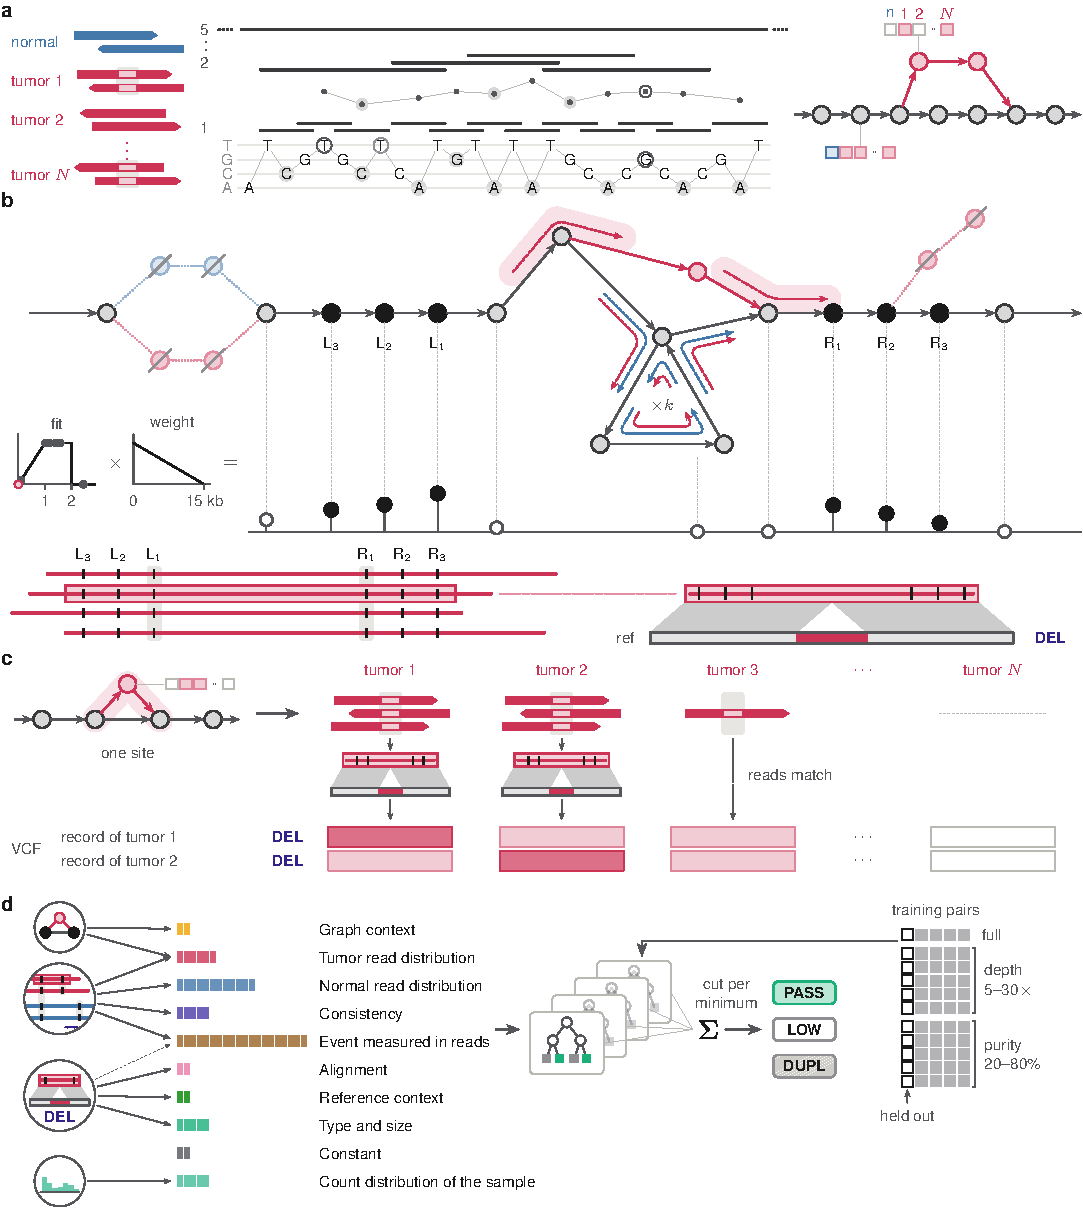
\includegraphics[width=\textwidth]{figures/fig_system.pdf}
\caption{Overview of \tool for one normal and $N$ tumor samples. (a) The reads are parsed into LCP cores, which form a single graph with a read count per sample at each node. (b) After sequencing-error bubbles and tips are removed, a site is a pair of edges traversed by tumor reads but not by normal reads; snippets of at most four tumor reads around its anchors are aligned. (c) A site is defined once for all tumors, and each tumor with enough reads at the site gets its own VCF record; light cells: carriers found from reads spanning the site. (d) Gradient-boosted trees mark each record PASS or LOW; duplicates are marked DUPL.}
\label{fig:overview}
\end{figure}

\paragraph{Core extraction.}
\tool homopolymer-compresses each read and partitions both strands into level-5 LCP cores using LCPtools~\cite{lcpan}, indexing each core by a 64-bit sequence hash that serves as its graph node identifier. 

\paragraph{Graph construction.}
% CAN: considering to move most of the details to supplementary.
For each sample, \tool counts each core and each pair of consecutive cores on the same strand of a read, skipping pairs of identical cores and cores that overlap the first or last 10\,bp of a read.
We denote the normal sample by $S_0$, the tumor samples by $S_1,\dots,S_N$, and the count of core $x$ in $S_s$ by $c_s(x)$.
\tool keeps a core in sample $S_s$ only if $c_s(x)\geq m_s$, which removes the noise of sequencing errors, as erroneous cores occur in few reads.
The minimum read support $m_s$ is 2 or 3, chosen from the counts of the sample.
In a tumor sample $S_t$, a core with $c_t(x)\geq 2$ is \emph{shared} if $c_0(x)\geq m_0$ and \emph{tumor-only} otherwise.
\tool sets
\par\noindent
\begin{minipage}{0.47\textwidth}
\begin{equation}
m_0=\begin{cases}2 & \text{if } \displaystyle\operatorname*{median}_{x:\,c_0(x)\geq 3} c_0(x)<\tau_{\mathrm{normal}},\\ 3 & \text{otherwise,}\end{cases}
\end{equation}
\end{minipage}\hfill
\begin{minipage}{0.51\textwidth}
\begin{equation}
m_t=\begin{cases}2 & \text{if } \displaystyle\operatorname*{P_{95}}_{\substack{x:\,c_t(x)\geq 3,\\ c_0(x)<m_0}} c_t(x)<\tau_{\mathrm{tumor}},\\ 3 & \text{otherwise,}\end{cases}
\end{equation}
\end{minipage}
\par\noindent
where the median grows with the depth of the normal sample, and the 95$^{th}$ percentile $\mathrm{P}_{95}$ of the tumor-only counts is high only when the tumor sample is both deep and pure.
We selected $\tau_{\mathrm{normal}}=20$ and $\tau_{\mathrm{tumor}}=20$ in our experiments, based on a parameter sweep over the CASTLE runs (Section~\ref{supsec:thresholds}).
\tool then builds a graph $G_s=(V_s,E_s)$ for each sample, with $V_s=\{x : c_s(x)\geq m_s\}$ and an edge $(u,v)\in E_s$ for each counted pair $(u,v)$ with $u,v\in V_s$, and merges these graphs into the case graph $G=(V,E)$ with $V=\bigcup_{s=0}^{N}V_s$ and $E=\bigcup_{s=0}^{N}E_s$, in which each node keeps its counts $c_s(x)$.
An edge is \emph{novel} if it is not in $E_0$ but is in some $E_t$ with at least $m$ occurrences in $S_t$, where $m=m_t$ in a pairwise run and $m=\min_t m_t$ in a joint run.
On either strand, a read is the sequence of its cores that are nodes of $G$, and it traverses each edge $(u,v)\in E$ whose endpoints are consecutive in this sequence.

From the cores that meet the minimum read support, \tool computes four summary metrics to capture the depth and purity of each pair.
Letting $\mu_t$ and $\mu_0$ denote the median counts of shared cores in the tumor and normal samples, respectively, these metrics comprise $\log_2\mu_t$, $\log_2\mu_0$, and the 5$^{th}$ and 95$^{th}$ percentiles of tumor-only core counts normalized by $\mu_t$.

\paragraph{Removal of sequencing errors and small variants.}
A node is \emph{branching} if it has multiple incoming or outgoing edges, while a \emph{chain} is a maximal non-branching path $x_1,\dots,x_\ell$ ($\ell \ge 2$). 
To eliminate sequencing errors, SNVs, and small indels, \tool prunes tips and bubbles from the graph  (Section~\ref{supsec:errors}).
This pruning strategy filtered 2.2--6.2 million nodes per pair into the removed set $R \subset V$ across the CASTLE pairs (Table~\ref{suptab:steps}).


\paragraph{SV site detection.}
Because a somatic SV often joins pre-existing genomic cores rather than creating novel nodes in the graph, it manifests as a tumor-specific path through nodes shared with the normal sample.
To detect these events, \tool identifies pairs of edges, termed \emph{sites}, that are traversed only by tumor reads.

Let $X$ denote the endpoints of unpruned novel edges $(u, v)$ where $u, v \notin R$.
We define a \emph{locus} as either a branching node in $X$ or a chain that contains a node in $X$.
A read crossing a locus defines a site $\sigma$ through the edges it enters and leaves:
\begin{equation}
\sigma =
\begin{cases}
\bigl((u,v),\,(v,w)\bigr) & \text{for consecutive cores } u, v, w,\\[2pt]
\bigl((u,x_1),\,(x_\ell,w)\bigr) & \text{for consecutive cores } u, x_1,\dots,x_\ell, w.
\end{cases}
\end{equation}
% MUTI: Note - S_0 is already defined as Sample-0 above. DO NOT OVERLOAD terms. I changed it to N to differentiate
Reads that begin or end within a chain do not form a site.
Letting $\mathcal{N}_0$ denote the set of normal read sites, \tool retains a candidate site $\sigma$ if its nodes avoid $R$ and it satisfies $\sigma \notin \mathcal{N}_0$ and $\max_{1\le s\le N} n_s(\sigma) \ge m$, where $n_s(\sigma)$ is the read count in tumor sample $s$.

For every retained site, \tool records $n_s(\sigma)$ across all tumor samples.
For each tumor sample reaching the support threshold ($n_s(\sigma) \ge m$), \tool designates a \emph{central read} $r$ that maximizes $\min(a_r, b_r)$, placing the site farthest from the read ends with $a_r$ and $b_r$ flanking bases.

\junk{
A somatic SV often creates no core that is new relative to the normal sample, because it joins cores that also occur elsewhere in the genome, so its nodes are shared with the normal sample and only the path of the reads through them differs. \tool searches for pairs of edges, called sites, that are traversed together by tumor reads only.

Let $X$ be the set of endpoints of novel edges $(u,v)$ with $u,v\notin R$. A locus is a branching node $v\in X$ or a chain $x_1,\dots,x_\ell$ with a node in $X$. A site $\sigma$ is the pair of edges by which a read enters and leaves a locus:
\begin{equation}
\sigma =
\begin{cases}
\bigl((u,v),\,(v,w)\bigr) & \text{if the read contains } u,v,w \text{ consecutively,}\\[2pt]
\bigl((u,x_1),\,(x_\ell,w)\bigr) & \text{if the read contains } u,x_1,\dots,x_\ell,w \text{ consecutively.}
\end{cases}
\end{equation}
A read that starts or ends inside a chain has no site there. Let $S_0$ be the sites of the normal reads, collected before the tumor reads are counted, and $n_s(\sigma)$ the number of reads of tumor sample $s$ with site $\sigma$. A site is kept if none of the nodes of its two edges is in $R$ and
\begin{equation}
\sigma\notin S_0 \quad\text{and}\quad \max_{1\leq s\leq N} n_s(\sigma)\geq m;
\end{equation}
from here on, ``site'' means a kept site. At a branching node $v$ that is not the first or last node of a chain, a read of tumor sample $s$ counts towards $n_s(\sigma)$ only if $v$ is also branching in the graph restricted to $V_0\cup V_s$. A branching caused only by the nodes of other tumor samples creates no site for sample $s$.

A site stores $n_s(\sigma)$ for all tumor samples and, for each tumor sample with $n_s(\sigma)\geq m$, a central read: the read $r$ with the site farthest from the read ends, which maximizes $\min(a_r,b_r)$, where $a_r$ and $b_r$ are the numbers of bases of $r$ before and after the cores of the site.
}

\paragraph{Snippet selection.}
\tool maps each candidate site to the reference by extracting a read snippet from the central read $r$ of tumor sample $t$, bounded by flanking anchors.
Let $d(x)$ be the distance from core $x$ on $r$ to the site boundary.
An anchor must occur uniquely on $r$, appear in both samples, and satisfy $c_0(x)\le 2\mu_0$, $c_t(x)\le 2\mu_t$, and $d(x)<15$\,kb.
On each flank, \tool selects up to three candidate anchors that maximize:
\begin{equation}
\mathrm{score}(x)=\sqrt{\min\!\Bigl(1,\frac{c_0(x)}{\mu_0}\Bigr)\cdot\min\!\Bigl(1,\frac{c_t(x)}{\mu_t}\Bigr)}\;\cdot\;\Bigl(1-\frac{d(x)}{15{,}000}\Bigr),
\label{eq:score}
\end{equation}
penalizing cores that are distant or poorly supported.
If a flank lacks eligible cores, \tool defaults to the site's outermost core.


\paragraph{Alignment of the snippets.}
\tool aligns snippets with minimap2~\cite{Li_2018} to short candidate reference windows rather than the whole genome (Section~\ref{supsec:align}).
It then aligns any remaining unaligned segments (50\,bp to 20\,kb) across the whole genome to resolve distal breakpoints of translocations and non-local insertions.

\vspace*{-0.3cm}
\paragraph{SV signatures and records.}
\tool extracts SV signatures from split alignments and from internal indels of at least 50\,bp, discarding any alignment with mapping quality below 10.
Following Severus~\cite{severus}, each signature comprises two oriented breakpoint coordinates on the reference (Section~\ref{supsec:signatures}).
Within each tumor sample, it then merges signatures of identical type and orientation with breakpoints that match within 50\,bp into a single record (Section~\ref{supsec:records}).

\vspace*{-0.3cm}
\paragraph{Read-level evidence.}
To determine whether normal reads also harbor a candidate SV, \tool inspects raw reads directly using the site's anchors.
For a read $x$ thar carries left and right anchors $A$ and $B$ at positions $p_x(A)$ and $p_x(B)$, we define the anchor distance as $\Delta_x = p_x(B) - p_x(A)$.
This distance matches the central read's distance $\Delta_r$ on reads supporting the tumor allele, but shifts by approximately the SV size on alternative alleles.
In a single pass across all reads, \tool calculates
%\begin{equation}
$D_x = \Delta_x - \Delta_r$,
%\end{equation}
classifying reads with $|D_x| < 20$\,bp as supporting the tumor allele; matching normal reads signal germline variation.
Because initial anchors may lie kilobases away, \tool repeats this distance measurement using refined anchors closer to the event (Section~\ref{supsec:evidence}).

\vspace*{-0.3cm}
\paragraph{Classification.}
Each record incorporates 56 features, including tumor read support, normal read $D_x$ distributions, local tumor-specific node counts, and mapping quality (Section~\ref{supsec:records}).
To account for coverage and tumor purity, \tool normalizes the 11 $\log_2$-count features by subtracting $\log_2(\mu_t+1)$ from tumor read or snippet counts and $\log_2(\mu_0+1)$ from normal read counts.
Adding $m$ and the four depth/purity metrics to these features gives 61 input features per record.

In a post-processing step, \tool classifies candidate records from the VCF using gradient-boosted decision trees~\cite{friedman,sklearn}.
Two records of one tumor sample are duplicates if both breakpoints of one lie within 500\,bp of those of the other, unless they have the same type and different orientations.
In each duplicate pair, \tool marks as DUPL the record with fewer supporting tumor reads before classification and the record with the lower predicted probability after it; DUPL records are not used for training.
We trained a single model across full-depth, downsampled, and 20--80\% purity configurations, enabling it to generalize across variable depths and purities.
\tool marks a record as PASS if its predicted probability meets a support-dependent threshold ($m$) selected via held-out validation on the training pairs (Sections~\ref{supsec:classifier} and~\ref{supsec:clseval}).

\vspace*{-0.3cm}
\paragraph{Joint calling of multiple tumors.}
In joint runs, \tool initially generates and classifies records separately for each tumor using sample-specific counts, then refines calls post-classification.
It clusters non-duplicate records across samples into a shared SV if the corresponding breakpoints match within 500\,bp on the same chromosomes.
Letting $\tau_s$ denote the probability threshold for sample $S_s$ (Section~\ref{supsec:classifier}), \tool accepts a record with probability $p$ if $p \ge \tau_s + 0.2$, or if $p \ge 0.1$ while another tumor sample supports the same SV with $p \ge \tau_{s'}$.
For an accepted SV, \tool rescues an uncalled tumor sample as a carrier if (i) at least three other tumors report candidate records, (ii) at least one spanning read supports the event ($|D_x| < 20$\,bp), and (iii) supporting reads comprise at least 25\% of its spanning coverage.
From the carrier sets of these calls, \tool builds a neighbor-joining tree~\cite{nj} of the tumor samples and re-decides the carriers of each SV with it: every side of every edge of the tree is a candidate carrier set, scored by the summed evidence of its members ($\operatorname{logit} p_k - \operatorname{logit} \tau_k$ for a tumor $k$ with a record of the SV, $-\mu$ with $\mu=0.5$ otherwise) plus a prior from the number of SVs whose carriers are exactly that set; if the best candidate scores above zero, its members without an accepted record become carriers of the SV, and carriers outside it are dropped (Section~\ref{supsec:joint}).

% MUTI: THIS PARAGRAPH BELONGS TO RESULTS
\junk{
\paragraph{Datasets and benchmarking.}
The real read sets (Section~\ref{supsec:datasets}) were analyzed against GRCh38. The other PacBio HiFi callers ran on minimap2 alignments of the same reads (Section~\ref{supsec:tools}), and the consensus sets were built with Minda (Section~\ref{supsec:consensus}). The simulated dataset and its truth sets are described in Sections~\ref{supsec:simgen} and~\ref{supsec:simeval}. Bootstrap 95\% intervals of the difference in F1 score between \tool and the best other caller were computed from 2,000 resamples, in which the consensus SVs of each pair were resampled with replacement for recall and the calls for precision, and the difference was averaged over the pairs; the two-sided $p$-value is twice the smaller fraction of resampled differences at or below and at or above zero. The $p$-values are not corrected for multiple testing.
}